%%%%%%%%%%%%%%%%%%%%%%%%%%%%%%%%%%%%%%%%%
% Beamer Presentation
\special{dvipdfmx:config z 0}
\documentclass[aspectratio=1610]{beamer}
%\usepackage[utf8]{inputenc}
%\usepackage[UTF8]{ctex}
%\usepackage{xeCJK}
\usepackage{pre}

\usepackage{tikz}
\usetikzlibrary{graphs, positioning, quotes, shapes.geometric, arrows.meta, chains,	matrix,	positioning, calc}

\usepackage{subfigure}

\DeclareMathOperator{\reg}{\mathrm{reg}}
\DeclareMathOperator{\ort}{\mathrm{ortho}}
\DeclareMathOperator{\no}{\mathrm{NO}}
\DeclareMathOperator{\eff}{\mathrm{eff}}


\numberwithin{equation}{section}
\setcounter{tocdepth}{2} % Show sections + subsections

\usepackage{hyperref}
\hypersetup{
	colorlinks=true,
	linkcolor=blue,
	filecolor=blue,      
	urlcolor=blue,
	citecolor=cyan,
	%pdfborder=001,
}

\usepackage{listings}
%\newcounter{lem}[section]\setcounter{lem}{0}
%\renewcommand{\thelem}{\arabic{section}.\arabic{lem}}
\newenvironment{mylemm}[2]{%
	%\refstepcounter{lem}%
	\ifstrempty{#2}
	{\newcommand{\mycol}{green!20}}
	{\newcommand{\mycol}{#2}}
	\mdfsetup{%
			frametitle={%
				\tikz[baseline=(current bounding box.east),outer sep=0pt]
				\node[anchor=east,rectangle,fill=\mycol]
				{\strut ~#1};}}%
	%
	\mdfsetup{innertopmargin=10pt,linecolor=\mycol,%
		linewidth=2pt,topline=true,%
		frametitleaboveskip=\dimexpr-\ht\strutbox\relax
	}
	\begin{mdframed}[]\relax%
		%\label{#2}
	}{\end{mdframed}}

%\usepackage{nicematrix}
\usepackage{threeparttable}



\usepackage[isbn=false,doi=false,url=false,
%hyperref=true,
uniquename=init,minnames=2,maxnames=4,
style=chem-acs]{biblatex}
%\addbibresource{emp2.bib}
%\addbibresource{casdft.bib}
%\addbibresource{mcpdft.bib}
\newcommand{\hf}[1]{\hfill{\footnotesize{#1}}}
%----------------------------------------------------------------------------------------
%	TITLE PAGE
%----------------------------------------------------------------------------------------

\title[]{%Work Report\\
%\vspace{15pt}
\textbf{Plotting Tutorial with matplotlib and Mathematica}
\vspace{15pt}} % The short title appears at the bottom of every slide, the full title is only on the title page

\author{Shirong Wang} % Your name
\institute[] % Your institution as it will appear on the bottom of every slide, may be shorthand to save space
{Department of Chemistry,
Fudan University \\ % Your institution for the title page
%\medskip
%\textit{} % Your email address
%Advisor: Prof. Xin Xu
}
\date{\today} % Date, can be changed to a custom date

\begin{document}

\begin{frame}
\titlepage % Print the title page as the first slide
\end{frame}

\begin{frame}
\frametitle{Overview} % Table of contents slide, comment this block out to remove it
\tableofcontents % Throughout your presentation, if you choose to use \section{} and \subsection{} commands, these will automatically be printed on this slide as an overview of your presentation
\end{frame}

%----------------------------------------------------------------------------------------
%	PRESENTATION SLIDES
%----------------------------------------------------------------------------------------
\section{Introduction}
\begin{frame}{Why matplotlib}
	\begin{itemize}
		\item Free and open source
		\item General and flexible
		\item Data execution with python
	\end{itemize}
	
\end{frame}

\section{matplotlib: A Simple Way}
\begin{frame}
Installation:
\begin{itemize}
	\item Anaconda for Linux/MacOS/Windows, latest version 2020.11\\
	\href{https://www.anaconda.com/products/individual}{www.anaconda.com/products/individual}\\
	\href{http://mirrors.nju.edu.cn/anaconda/archive}{mirrors.nju.edu.cn/anaconda/archive}
	   \item pip, apt, pacman, ...
	\item IDE: Spyder, VS Code, Jupyter notebook
\end{itemize}

\end{frame}

\begin{frame}{Get Started with IDE}
	\begin{figure}
		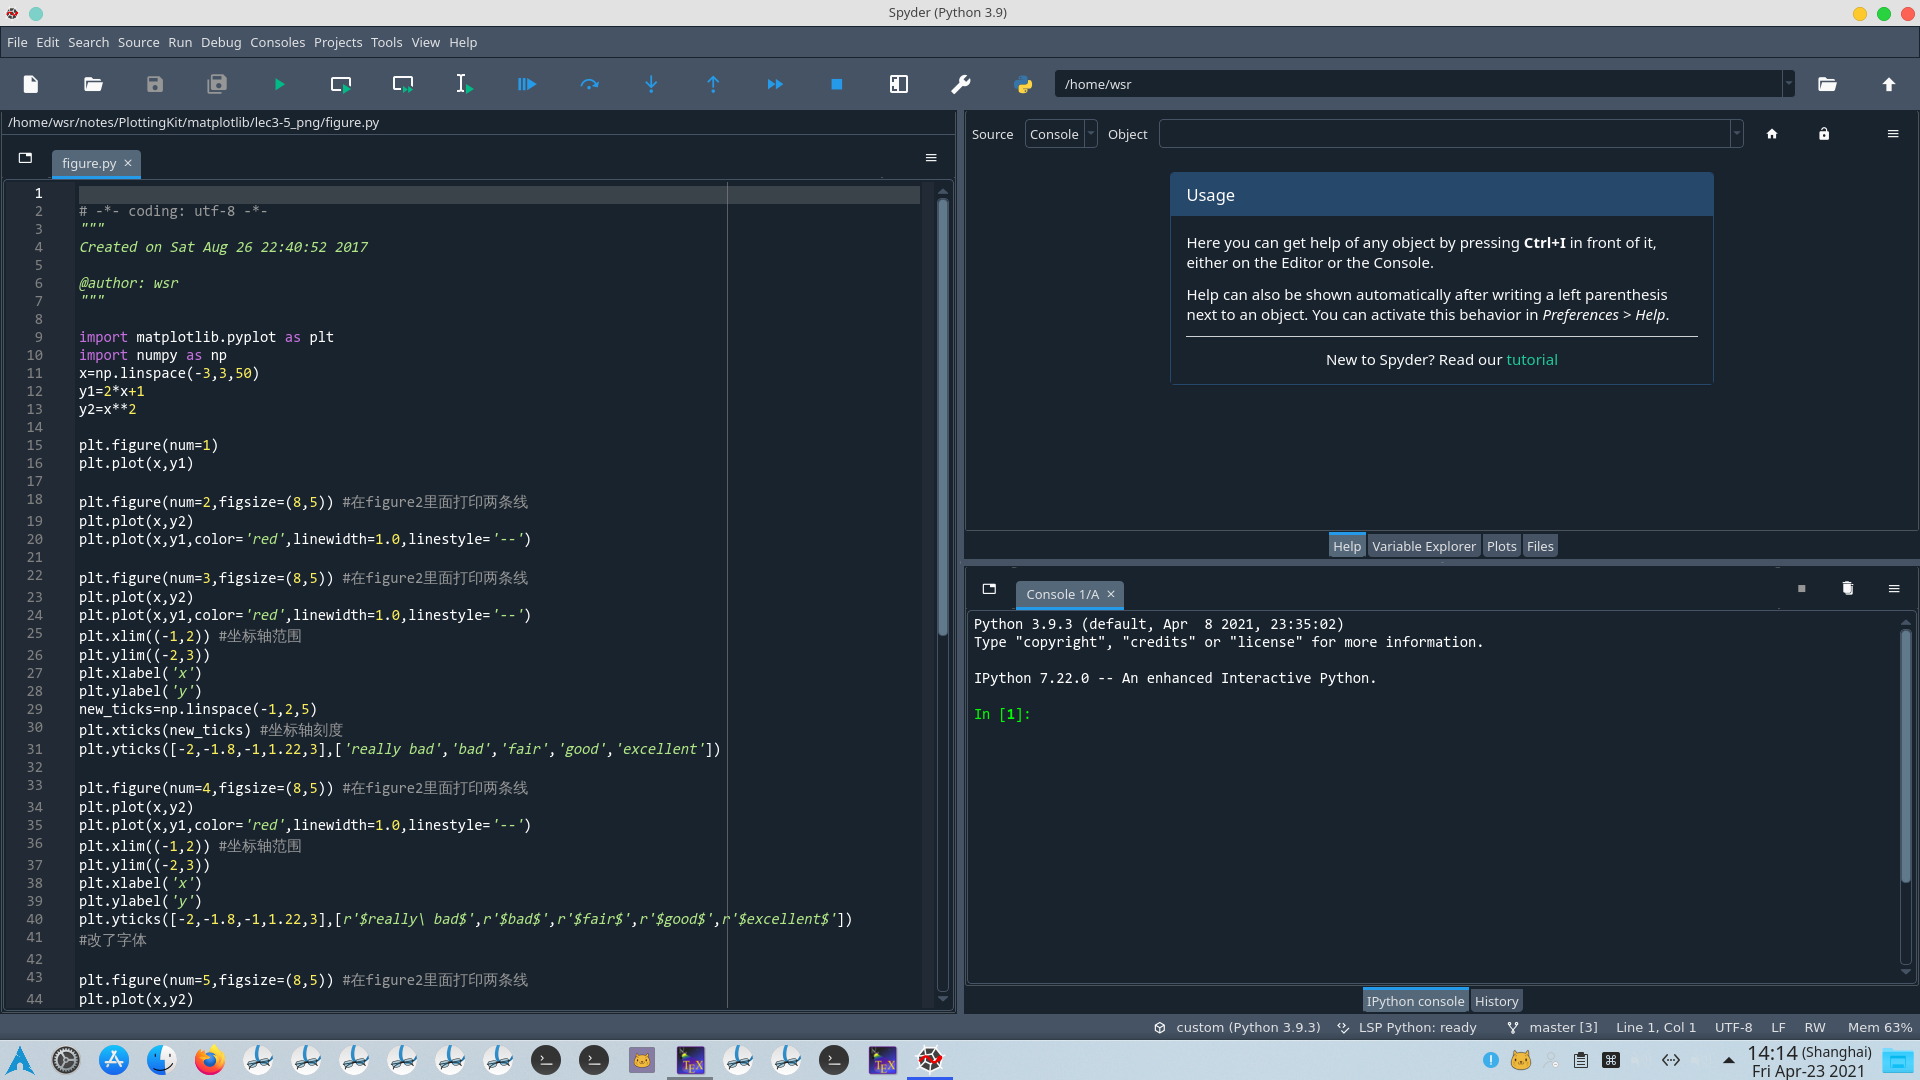
\includegraphics[width=0.9\linewidth]{spyd.png}
	\end{figure}
\end{frame}

\begin{frame}{Get Started with IDE}
	\begin{figure}
		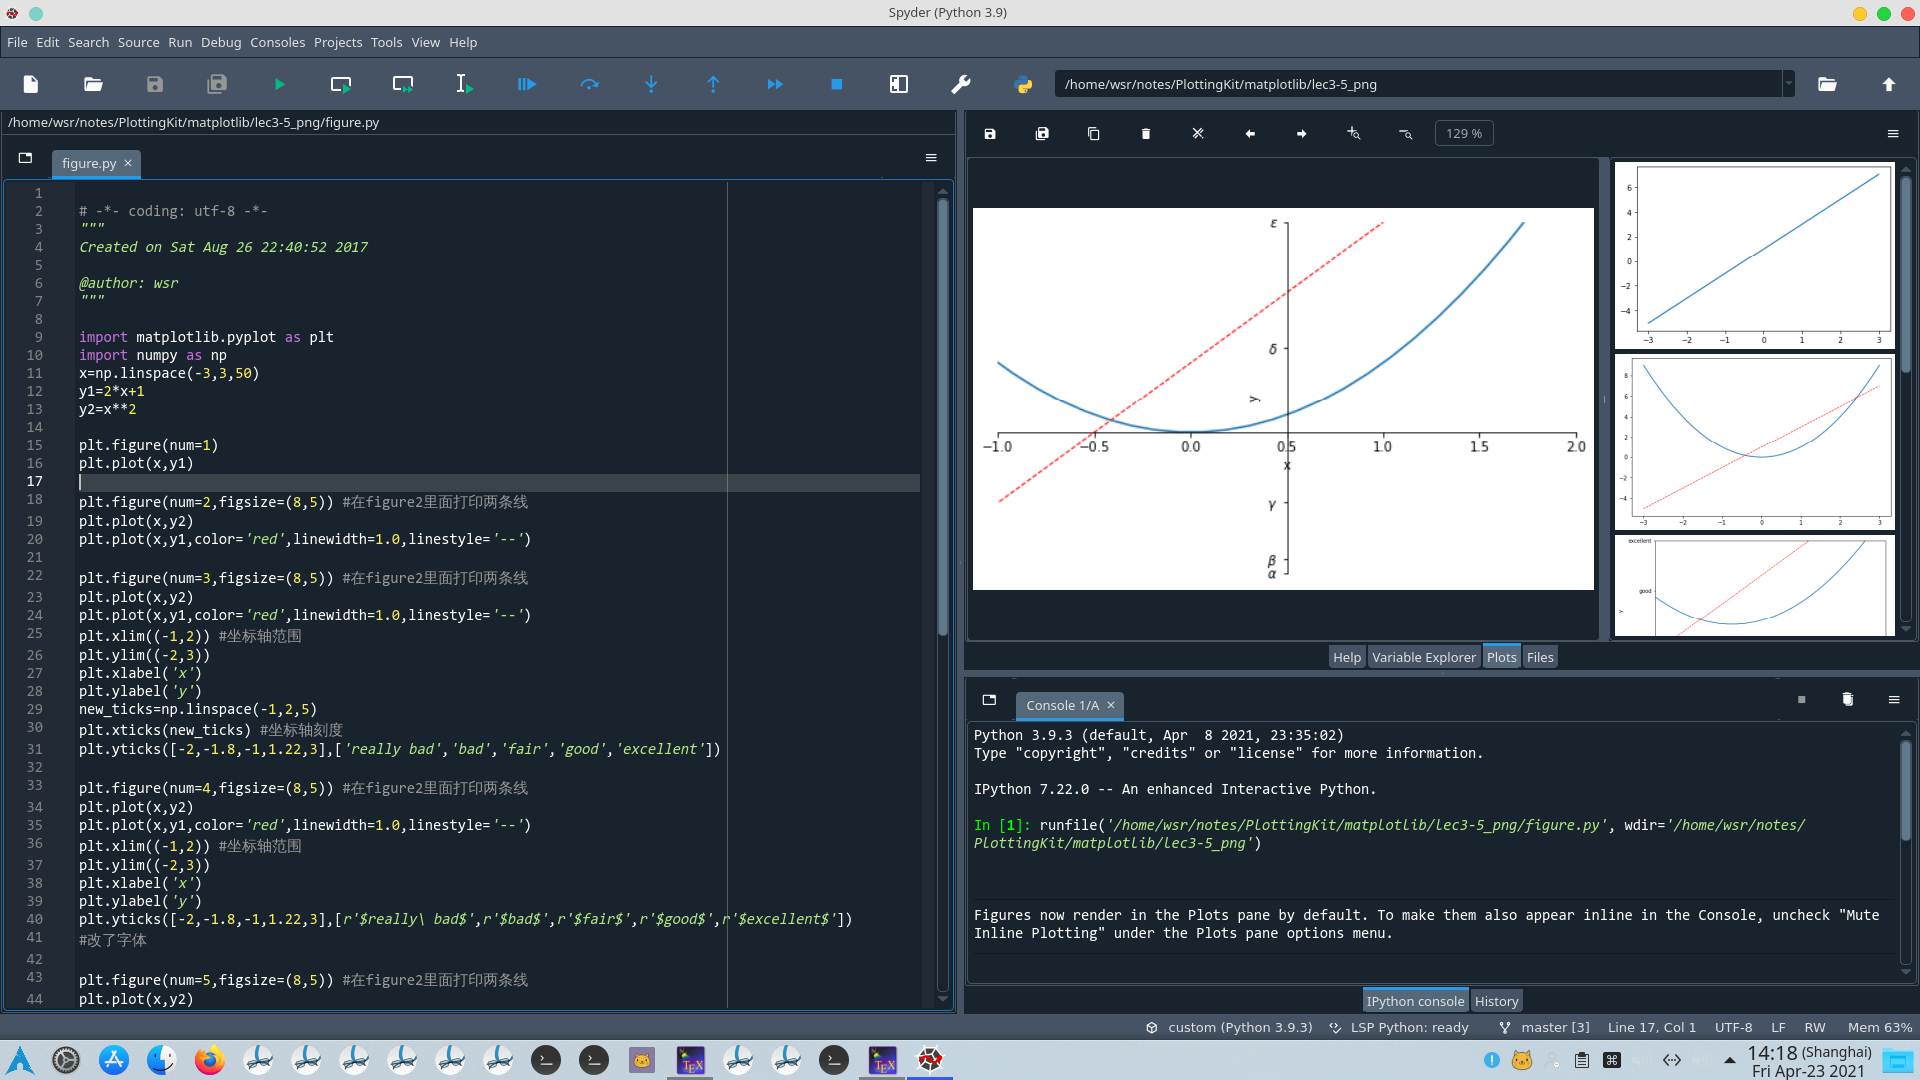
\includegraphics[width=0.9\linewidth]{spyd2.png}
	\end{figure}
\end{frame}

\section{matplotlib: A Hard Way}

\section{Mathematica}


\begin{frame}
~\vspace{50pt}\\
\centering{\LARGE Thank You}



\end{frame}


%\iffalse
%\begin{frame}
%
%\end{frame}
%\fi
%\bibliography{pre1}
%\bibliographystyle{plain}




\end{document} 